\NeedsTeXFormat{LaTeX2e}
\documentclass[a4paper,12pt,
headsepline,        % Linie Kopfzeile / Text
oneside,            % einseitig
bibtotoc,           % Lit.verz. ins Inh.verz.
pointlessnumbers,   % kein Punkt nach letzter Gliederungsziffer
%DIV=15,              % Satzspiegel auf 15er Raster, schmalere Ränder   
BCOR15mm             % mehr li. Rand zum Binden der Arbeit
%,draft
]{scrbook}
\KOMAoptions{DIV=last}

\pagestyle{headings}
\usepackage{blindtext}

% für Texte in deutscher Sprache
\usepackage[ngerman]{babel}
\usepackage[utf8]{inputenc}
\usepackage[T1]{fontenc}

% Helvetica als Standard-Dokumentschrift
\usepackage[scaled]{helvet}
\renewcommand{\familydefault}{\sfdefault} 

\usepackage{graphicx}

% Tabellen mit fester Gesamtbreite und variabler Spaltenbreite
\usepackage{tabularx} 
%\begin{tabularx}{Breite}    {Spaltendefinition} ... \end{tabularx}
%\begin{tabularx}{\textwidth}{XXl} ...               \end{tabularx}

\usepackage{url}              % \url{http://...} in Schreibmaschinenschrift
\usepackage{color}            % zum Setzen farbigen Textes
\usepackage{amssymb, amsmath} % Pakete für Mathe-Umgebungen und -Symbole


\usepackage{setspace} % Paket für div. Abstände, z.B. ZA
\setlength{\parindent}{0pt}
\setlength{\parskip}{1.4ex plus 0.35ex minus 0.3ex}

% Tiefe, bis zu der Überschriften in das Inhaltsverzeichnis kommen
\setcounter{tocdepth}{3} % ist Standard

% Beispiele für Quellcode
\usepackage{listings}
\lstset{language=Java,
  showstringspaces=false,
  frame=single,
  numbers=left,
  basicstyle=\ttfamily,
  numberstyle=\tiny}

% hier Namen etc. einsetzen
% TODO hier anpassen
\newcommand{\fullname}{Florian Krötz}
\newcommand{\email}{florian.kroetz@uni-ulm.de}
\newcommand{\titel}{Der Titel der Arbeit, meist länger als eine Zeile}
\newcommand{\jahr}{2017}
\newcommand{\matnr}{884948}
\newcommand{\gutachterA}{Prof.~Dr.~Streng Geheim}
\newcommand{\gutachterB}{Prof.~Dr.~Un Leserlich}
\newcommand{\betreuer}{Betreuername}

% hier die Fakultät auswählen
%\newcommand{\fakultaet}{---  Im Quellcode anpassen nicht vergessen! ---}
%\newcommand{\fakultaet}{Ingenieurwissenschaften, Informatik und Psychologie}
\newcommand{\fakultaet}{Mathematik und\\Wirtschafts-\\wissenschaften}
%\newcommand{\fakultaet}{Medizin}
%\newcommand{\fakultaet}{Naturwissenschaften}

% hier das Institut einsetzen
\newcommand{\institut}{--- Institut im Quellcode anpassen nicht vergessen! ---}

%color in tables
\usepackage{colortbl}
\definecolor{Gray}{rgb}{0.80784, 0.86667, 0.90196} %dunkelblau
\definecolor{Lightgray}{rgb}{0.9176, 0.95, 0.95686} %hellblau
\definecolor{Akzent}{rgb}{0.6627, 0.63529, 0.55294} %akzentfarbe
\setlength{\arrayrulewidth}{0.1pt}


\pdfinfo{
  /Author (\fullname)
  /Title (\titel)
  /Producer     (pdfeTex 3.14159-1.30.6-2.2)
  /Keywords ()
}

\usepackage{hyperref}
\hypersetup{
pdftitle=\titel,
pdfauthor=\fullname,
pdfsubject={Diplomarbeit},
pdfproducer={pdfeTex 3.14159-1.30.6-2.2},
colorlinks=false,
pdfborder=0 0 0	% keine Box um die Links!
}

%Trennungsregeln
\hyphenation{Sil-ben-trenn-ung}

\begin{document}
\frontmatter

% Titelseite
\thispagestyle{empty}
\begin{addmargin*}[4mm]{-10mm}


\includegraphics[height=1.8cm]{images/unilogo_bild}
\hfill

\includegraphics[height=1.8cm]{images/unilogo_wort}\\[1em]

{\footnotesize
%{\bfseries Universität Ulm} \textbar ~89069 Ulm \textbar ~Germany
\hspace*{115mm}\parbox[t]{35mm}{\bfseries Fakultät für\\
\fakultaet\\

\mdseries \institut}\\[2cm]

\parbox{140mm}{\bfseries \LARGE \titel}\\[2.5em]
{\footnotesize Bachelorarbeit an der Universität Ulm}\\[3em]

{\footnotesize \bfseries Vorgelegt von:}\\
{\footnotesize \fullname\\\email}\\[2em]
{\footnotesize \bfseries Gutachter:}\\                     
{\footnotesize\gutachterA\\
\gutachterB}\\[2em]
{\footnotesize \bfseries Betreuer:}\\ 
{\footnotesize\betreuer}\\\\
{\footnotesize\jahr}
}
\end{addmargin*}


% Impressum
\clearpage
\thispagestyle{empty}
{ \small
  \flushleft
  Fassung \today \\\vfill
  \copyright~\jahr~\fullname\\[0.5em]
% Wenn Sie Ihre Arbeit unter einer freien Lizenz bereitstellen möchten, können Sie die nächste Zeile in Ihren Code aufnehmen. Bitte beachten Sie, dass Sie hierfür an allen Inhalten, inklusive enthaltener Abbildungen, die notwendigen Rechte benötigen! Beim Veröffentlichungsexemplar Ihrer Dissertation achten Sie bitte darauf, dass der Lizenztext nicht den Angaben in den Metadaten der genutzten Publikationsplattform widerspricht. Nähere Information zu den Creative Commons Lizenzen erhalten Sie hier: https://creativecommons.org/licenses/
%This work is licensed under the Creative Commons Attribution 4.0 International (CC BY 4.0) License. To view a copy of this license, visit \href{https://creativecommons.org/licenses/by/4.0/}{https://creativecommons.org/licenses/by/4.0/} or send a letter to Creative Commons, 543 Howard Street, 5th Floor, San Francisco, California, 94105, USA. \\
  Satz: PDF-\LaTeXe
}


% ab hier Zeilenabstand etwas größer 
\setstretch{1.1}

%\onehalfspacing % nur dann, wenn gefordert; ist sehr groß!!

\tableofcontents

\mainmatter
% TODO Kapitel einbinden
\chapter{Einleitung}

Diese kleine Einleitung soll dem Nutzer helfen selbst die eigene Arbeit mit \LaTeX{} zu schreiben. Sie enth"alt Beispiele zu den wichtigsten Themen .

\blindtext

\section{Struktur}

Für diese Arbeit lassen sich als "Uberschriften die "Uberschriften in verschiedenen Stufen verwenden.

\begin{verbatim}
\chapter{Einleitung}
\section{Struktur}
\subsection{}
\subsubsection{}
\end{verbatim}

Allerdings sollte man sich überlegen, ob man wirklich bis zur Stufe \verb|subsubsection| "Uberschriften benötigt.



\section{Illustrationen}

\blindtext

\blindtext

\subsection{Bilder}

Bilder kann man natürlich auch integrieren und einfügen. Für Fotos und Ähnliches unterstützt PDF-\LaTeX{} direkt \verb|jpg| und \verb|png|, ansonsten empfiehlt es sich, Vektorgrafiken zu verwenden und diese als \verb|pdf| zu speichern. Sollte ein Bild einmal zu viel weißen Raum um sich haben, so kann man mit dem Werkzeug \verb|pdfcrop| das Bild automatisch zuschneiden\,\cite{pdfcrop}.

\begin{figure}[ht]
\centering
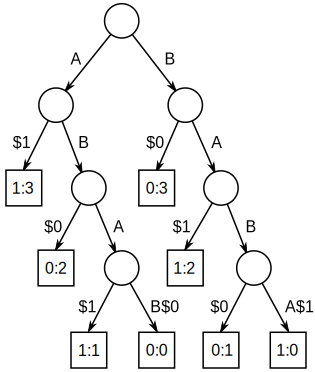
\includegraphics[width=.4\textwidth]{images/Suffix_tree_ABAB_BABA}
\caption{\label{fig:bild1}Beschreibung/Beschriftung des Bilds}
\end{figure}

Mit Hilfe eines Labels \verb|\label{fig:bild1}| kann man sich dann im fortlaufenden Text mittels eines Querverweises auf diese Grafik beziehen: \verb|\ref{fig:bild1}|. An der Stelle des ref-Kommandos platziert LaTeX die Nummer der Abbildung: \glq siehe Abbildung \ref{fig:bild1}\grq.


\subsection{Tabellen}

Seite \pageref{tab:beispieltabelle} enthält Beispieltabelle \ref{tab:beispieltabelle}. In jedem \LaTeX{}-Buch finden sich gute Anleitungen zum Erstellen von Tabellen. Komplexere Tabellen können in Excel vorgefertigt und mit einem Umwamdlungsprogramm oder -werkzeug nach LaTeX konvertiert werden.

\begin{table}[h]
\begin{center}
\begin{tabular}{|l|l|l|}
	A & B & C \\\hline
	x & x & x \\
	x & x & x
\end{tabular}
\end{center}
\caption{Eine kleine Beispieltabelle}
\label{tab:beispieltabelle}
\end{table}


\subsection{Formeln}

Mathematische Formeln lassen sich in der Umgebung  \verb|math| erzeugen. Die Kurz- Schreibweise lautet \verb|\( a^2+b^2=c^2 \)|;  hierbei steht die Formel dann im laufenden Text: \( a^2+b^2=c^2 \). Die kürzeste Form ist mit zwei \verb|$| um die Formel, z.B.~so: Wasser ist H$_2$O.

Mit der Schreibweise \verb|\[ y=x^2 \]| wird die Formel mittig in einer eigenen Zeile gesetzt, z.B.

\[y = x^2 \]

Formeln in der Umgebung \verb|equation| werden mittig in einer eigenen Zeile gesetzt und fortlaufend nummeriert:

\begin{equation}
x_{1,2} = \frac{-b\pm\sqrt{b^2-4ac}}{2a}
\label{mitternachtsformel}
\end{equation}
Wenn wir z.B.~über die beliebte Mitternachtsformel (Gleichung \ref{mitternachtsformel}) Details im umliegenden Text schreiben wollen, lässt sich diese wie ein Bild referenzieren.



\subsection{Quellcode}

Quellcode und ähnlich zu formatierende Texte können mit \verb|verbatim| in einer Umgebung gesetzt werden.

\begin{verbatim}
Dieser Text ist in Schreibmaschinenschrift
\end{verbatim}

Schöner geht es mit dem \verb|listings|-Paket, das Quelltext auch entsprechend formatiert. Dazu kann man in der Präambel die Sprache angeben, in der die Quellcodes geschrieben sind.

\begin{lstlisting}
public class Hello {
    public static void main(String[] args) {
        System.out.println("Hello World");
    }
}
\end{lstlisting}

Innerhalb einer Zeile gibt man Wörter am Besten als \verb|\verb##| an, dabei erwartet \LaTeX{} zweimal das gleiche Zeichen als Begrenzer. Im Beispiel ist dies die Raute \verb|#|, man kann aber ein anderes Zeichen nehmen, z.B. das Plus .



\section{Text}

Text kann mit dem Befehl \verb|\emph{}| \emph{hervorgehoben} werden. Falls in einem Satz ein Punkt vorkommt, macht man danach kein Leerzeichen sondern eine Tilde (\verb|z.~B.~so!|), denn dann fügt \LaTeX{} den korrekten Abstand ein, z.~B.~so!


In der Präambel der vorliegenden tex-Datei gibt es den Befehl \verb|hypenation|, der zur Silbentrennung da ist. \LaTeX{} verfügt zwar über  eine eingebaute Silbentrennung, die jedoch bei manchen Wörtern falsch trennt. Damit diese Wörter korrekt getrennt werden, gibt man sie dann mit dem Befehl in der Präambel an\footnote{Das Wort \emph{Silbentrennung} ist hier das Beispiel}.

Fußnoten werden mit dem Befehl \verb|footnote| mitten in den fortlaufenden Text eingefügt. \footnote{Wie man schon im vorherigen Absatz sehen konnte.}

In wissenschaftlichen Arbeiten muss man des öfteren andere Arbeiten zitieren. Dazu nutzt man den Befehl \verb|\cite{name}|. In eckigen Klammern kann man noch die Seitenzahl angeben, falls notwendig. Der Name ist ein Schlüssel aus der Datei \verb|bibliography.bib| \cite[S.~10]{kopka}. Falls einmal ein Werk nur indirekt zu einem Teil der Arbeit beigetragen hat, kann man es auch mit \verb|nocite| angeben, dann landet es in der Literaturliste, ohne dass es im Text ausdrücklich zitert wird.


\subsection{Weiterführendes}

Zum Schluss sei auf die Vielzahl an Büchern zu \LaTeX{} verwiesen. In jeder Bibliothek wird sich eine Einführung finden, in der dann weitere Themen wie mathematische Formeln, Aufbau von Briefen und viele nützliche Erweiterungen besprochen werden.


\chapter{Einleitung}

\section{Erste Schritte}
\begin{itemize}
	\item QR beschreiben
	\item Householder trans
	\item Matrix darstellung(inc row col bla)
	\item das ganze geblockt
	\item 
\end{itemize}

\subsection{Sonstiges}
\begin{itemize}
	\item LAPACK
	\item	
\end{itemize}

\section{Fragen}
\begin{enumerate}
	\item Wie testet man, ob Zerlegung $A=QR$ genau genug ist ?
	\item Apply $Q$
\end{enumerate} 

\section{Ziel}
\begin{align}
	A=QR\\
	\lVert Ax -b \rVert_2 \rightarrow \text{min}\\
	Q^Tb
\end{align}

\section{Ungeblockte $QR$ Zerlegung}
Input: $A \in m x n$\\
Output $A$ mit $R$ und Normalenvektoren $\tau$ 




\appendix
% TODO Anhänge einbinden
\chapter{Quelltexte}

In diesem Anhang sind einige wichtige Quelltexte aufgeführt.

\begin{lstlisting}
public class Hello {
    public static void main(String[] args) {
        System.out.println("Hello World");
    }
}
\end{lstlisting}


\backmatter
\nocite{Knappen2009}
\nocite{Mittelbach2005}
\nocite{Schlosser2014}
\nocite{Sturm2012}
\nocite{Voss2010}

%\bibliographystyle{plaindin} % Nummern und alphabetisch sortiert
%\bibliographystyle{alphadin} % Buchstaben und sortiert
\bibliographystyle{abbrvdin} % Nummern und abgekürzte Namen
%\bibliographystyle{unsrtdin} % Nummern und unsortiert
\bibliography{bibliography}


\clearpage
\thispagestyle{empty}

Name: \fullname \hfill Matrikelnummer: \matnr \vspace{2cm}

\minisec{Erklärung}

Ich erkläre, dass ich die Arbeit selbständig verfasst und keine anderen als die angegebenen Quellen und Hilfsmittel verwendet habe.\vspace{2cm}

Ulm, den \dotfill

\hspace{10cm} {\footnotesize \fullname}
\end{document}
